\documentclass{beamer} % [t] aligns itemize/enumerate lists at the top
\usetheme{Boadilla}
\usecolortheme{default}

\title{Automated Market-Making}
\author{Joshua Acton}
\date{22nd March 2024}
\subtitle{Supervised by Professor Nick Whiteley}

% Title slide
\begin{document}
\begin{frame}
    \titlepage
\end{frame}

% Introduction slide
\begin{frame}{Introduction}
    \begin{itemize}
    \item How do financial markets work at the level of individual participants?
    \item How can we use stochastic control theory to model the behaviour of market participants?
    \item The Avellaneda-Stoikov Model
    \item Results on the statistical properties of the limit orderbook
    \end{itemize}
\end{frame}

\begin{frame}{The limit orderbook}
    \begin{itemize}
        \item Can either place \emph{limit} orders or \emph{market} orders
        \item \emph{Limit} orders guaruntee price but not execution
        \begin{itemize}
            \item Limit orders can also be ammended/updated for as long as they exist
        \end{itemize}
        \item \emph{Market} orders guaruntee execution but not price
        \item \emph{Spread} between best bid and best ask $\rightarrow$ £0.02
        \item Can view the mid-price (here £1.00) as the ``true'' price
    \end{itemize}
    \begin{center}
        \begin{tabular}{ |c|c|c| } 
            \hline
            Side & Price /£ & Volume \\ 
            \hline
            A & 1.02 & 50 \\
            A & 1.01 & 30 \\
            \_ & 1.00 & 0 \\
            B & 0.99 & 25 \\ 
            B & 0.98 & 45 \\
            \hline
        \end{tabular}
    \end{center}
\end{frame}

\begin{frame}{The limit orderbook}
    After market buy order for 20 shares:
    \begin{center}
        \begin{tabular}{ |c|c|c| } 
            \hline
            Side & Price /£ & Volume \\ 
            \hline
            A & 1.02 & 50 \\
            A & 1.01 & \textcolor{red}{10} \\
            \_ & 1.00 & 0 \\
            B & 0.99 & 25 \\ 
            B & 0.98 & 45 \\
            \hline
        \end{tabular}
    \end{center}
    After another market buy order for 30 shares:
    \begin{center}
        \begin{tabular}{ |c|c|c| } 
            \hline
            Side & Price /£ & Volume \\ 
            \hline
            A & 1.02 & \textcolor{red}{30} \\
            A & 1.01 & \textcolor{red}{0} \\
            \_ & 1.00 & 0 \\
            B & 0.99 & 25 \\ 
            B & 0.98 & 45 \\
            \hline
        \end{tabular}
    \end{center}
\end{frame}

\begin{frame}{Dealer considerations}
    Problem:
    \begin{itemize}
        \item What if no one wants to sell? resp. buy?
        \item What if buyers and sellers have wildly different price expectations?
    \end{itemize}
    Idea:
    \begin{itemize}
        \item Simultaneously place bid and ask limit orders $\rightarrow$ simultaneously buying and selling
        \item Enables other market participants to always have someone to trade against $\rightarrow$ ``providing liquidity''
        \item Narrows the spread between bid and ask prices, decreasing implied cost of trading
        \item Dealer profits the small spread between buying and selling, multiplied across a large trading volume
    \end{itemize}
    Risk:
    \begin{itemize}
        \item Inventory
    \end{itemize}
\end{frame}

\begin{frame}{Modelling dealer behavior}
    If dealer accrues positive inventory:
    \begin{itemize}
        \item Want to sell more than buy
        \item Set lower ask price
    \end{itemize}
    If dealer accrues negative inventory:
    \begin{itemize}
        \item Want to buy more than sell
        \item Set a higher bid price
    \end{itemize}
    Now the maths\dots
\end{frame}

\begin{frame}{Stochastic Optimal Control}
    Following Pham (2009):

    System:
    \begin{equation}
        \mathrm dX_t=b(X_t,\alpha_t)\mathrm dt+\sigma(X_t,\alpha_t)\mathrm dW_t
    \end{equation}
    Objective (Finite time horizon):
    \begin{equation}
        v(t,x):=\sup_{\alpha\in\mathcal A}\mathbb{E}\left[\int_t^Tf(s,X_s^{t,x},\alpha_s)\mathrm ds+g(X_T^{t,x})\right]
    \end{equation}
    Dynamic Programming Principle:
    \begin{equation}
        v(t,x)=\sup_{\alpha\in\mathcal A}\mathbb{E}\left[\int_t^\theta f(s,X_s^{t,x},\alpha_s)\mathrm ds+v(\theta,X_\theta^{t,x})\right]
    \end{equation}
    Hamilton-Jacobi-Bellman Equation:
    \begin{equation}
        \frac{\partial v}{\partial t}(t,x)+\sup_{\alpha\in\mathcal{A}}\left[\mathcal{L}^\alpha v(t,x)+f(t,x,\alpha)\right]=0,\;v(T,x)=g(x)
    \end{equation}
\end{frame}

\begin{frame}{The Avellaneda-Stoikov model}
    Following Avellaneda \& Stoikov (2008):

    Model market mid-price as Brownian motion with variance $\sigma^2$ (no drift)
    $$\mathrm d S_t=\sigma \mathrm d W_t,\;t\in[0,T]$$
    The dealer quotes bid $p^b$ and ask $p^a$ with spreads $\delta^b=s-p^b$ and $\delta^a=p^a-s$
    respectively.
    We assume that 
    \begin{itemize}
        \item Market buy orders `lift' the dealer's sell orders at Poisson rate $\lambda^a(\delta^a)$
        \item Market sell orders `hit' the dealer's bid orders at Poisson rate $\lambda^b(\delta^b)$
        \item $\lambda$ is a decreasing function of $\delta$
    \end{itemize}
    Have stochastic wealth and inventory:
    \begin{equation}
        \mathrm dX_t=p^a\mathrm dN_t^a-p^b\mathrm dN_t^b
    \end{equation}
    \begin{equation}
        q_t=N_t^b-N_t^a
    \end{equation}
\end{frame}

\begin{frame}{The Avellaneda-Stoikov model}
    Objective function: Maximise expected utility of terminal wealth over possible bid/ask spreads $\delta^a,\delta^b$
    \begin{equation}
        u(s,x,q,t)=\max_{\delta^a,\delta^b}\mathbb{E}\left[-e^{-\gamma(X_T+q_TS_T)}|\mathcal{F}_t\right]
    \end{equation}
    \begin{itemize}
        \item HJB equation very difficult, maybe impossible, to solve analytically
        \item Through some asymptotic approximations we can work out an approximate solution in terms of our model paramaters
    \end{itemize}
\end{frame}

\begin{frame}{The Avellaneda-Stoikov model}
    We obtain the dealer's reservation price
    \begin{equation}
        r(s,q,t)=s-q\gamma\sigma^2(T-t)
    \end{equation}
    which reflects a shift to the mid-price depending on our current inventory and model parameters, and our quote spread
    \begin{equation}
        \delta^a+\delta^b=\gamma\sigma^2(T-t)+\frac{2}{\gamma}\log\left(1+\frac{\gamma}{k}\right)
    \end{equation}
    with $\gamma$ and $\sigma$ as before, $k$ is a parameter from the orderbook describing how 
    market order size impacts prices.
\end{frame}

\begin{frame}{Statistical properties of the limit order book}
    Poisson intensity $\lambda(\delta)$ describes how likely a limit order is to be executed as a function of it's 
    distance to the mid-price. Need some statistics regarding:
    \begin{itemize}
        \item Overall frequency of market orders
        \begin{itemize}
            \item For simplicity, assume constant $\Lambda$
        \end{itemize}
        \item Size distribution of market orders
        \begin{itemize}
            \item Power law $f_Q(x)\propto x^{-1-a}$
        \end{itemize}
        \item Price impact of large market orders
        \begin{itemize}
            \item Either $\Delta p\propto Q^\beta$ or $\Delta p\propto\log Q$
        \end{itemize}
    \end{itemize}
    Using the second result for price impact we obtain:
    \begin{align*}
        \lambda(\delta)=\Lambda\mathbb{P}(\Delta p>\delta)&=\Lambda\mathbb{P}(\log Q>K\delta)\\
        &=\Lambda\mathbb{P}\left(Q>e^{K\delta}\right)\\
        &=\Lambda\int_{e^{K\delta}}^{\infty}x^{-1-a}dx\\
        &=Ae^{-ka\delta}
    \end{align*}
\end{frame}

\begin{frame}{The Avellaneda-Stoikov model - Summary}
    \begin{itemize}
        \item Estimate parameters from market data
    \end{itemize}
    At each timestep, given current inventory and estimated parameters:
    \begin{itemize}
        \item Compute reservation price $r(s,q,t)$
        \item Compute spread $\delta^a+\delta^b$
        \item Set quotes $p^a=r(s,q,t)+\frac{\delta^a+\delta^b}{2}$, $p^b=r(s,q,t)-\frac{\delta^a+\delta^b}{2}$
    \end{itemize}
    \center{
        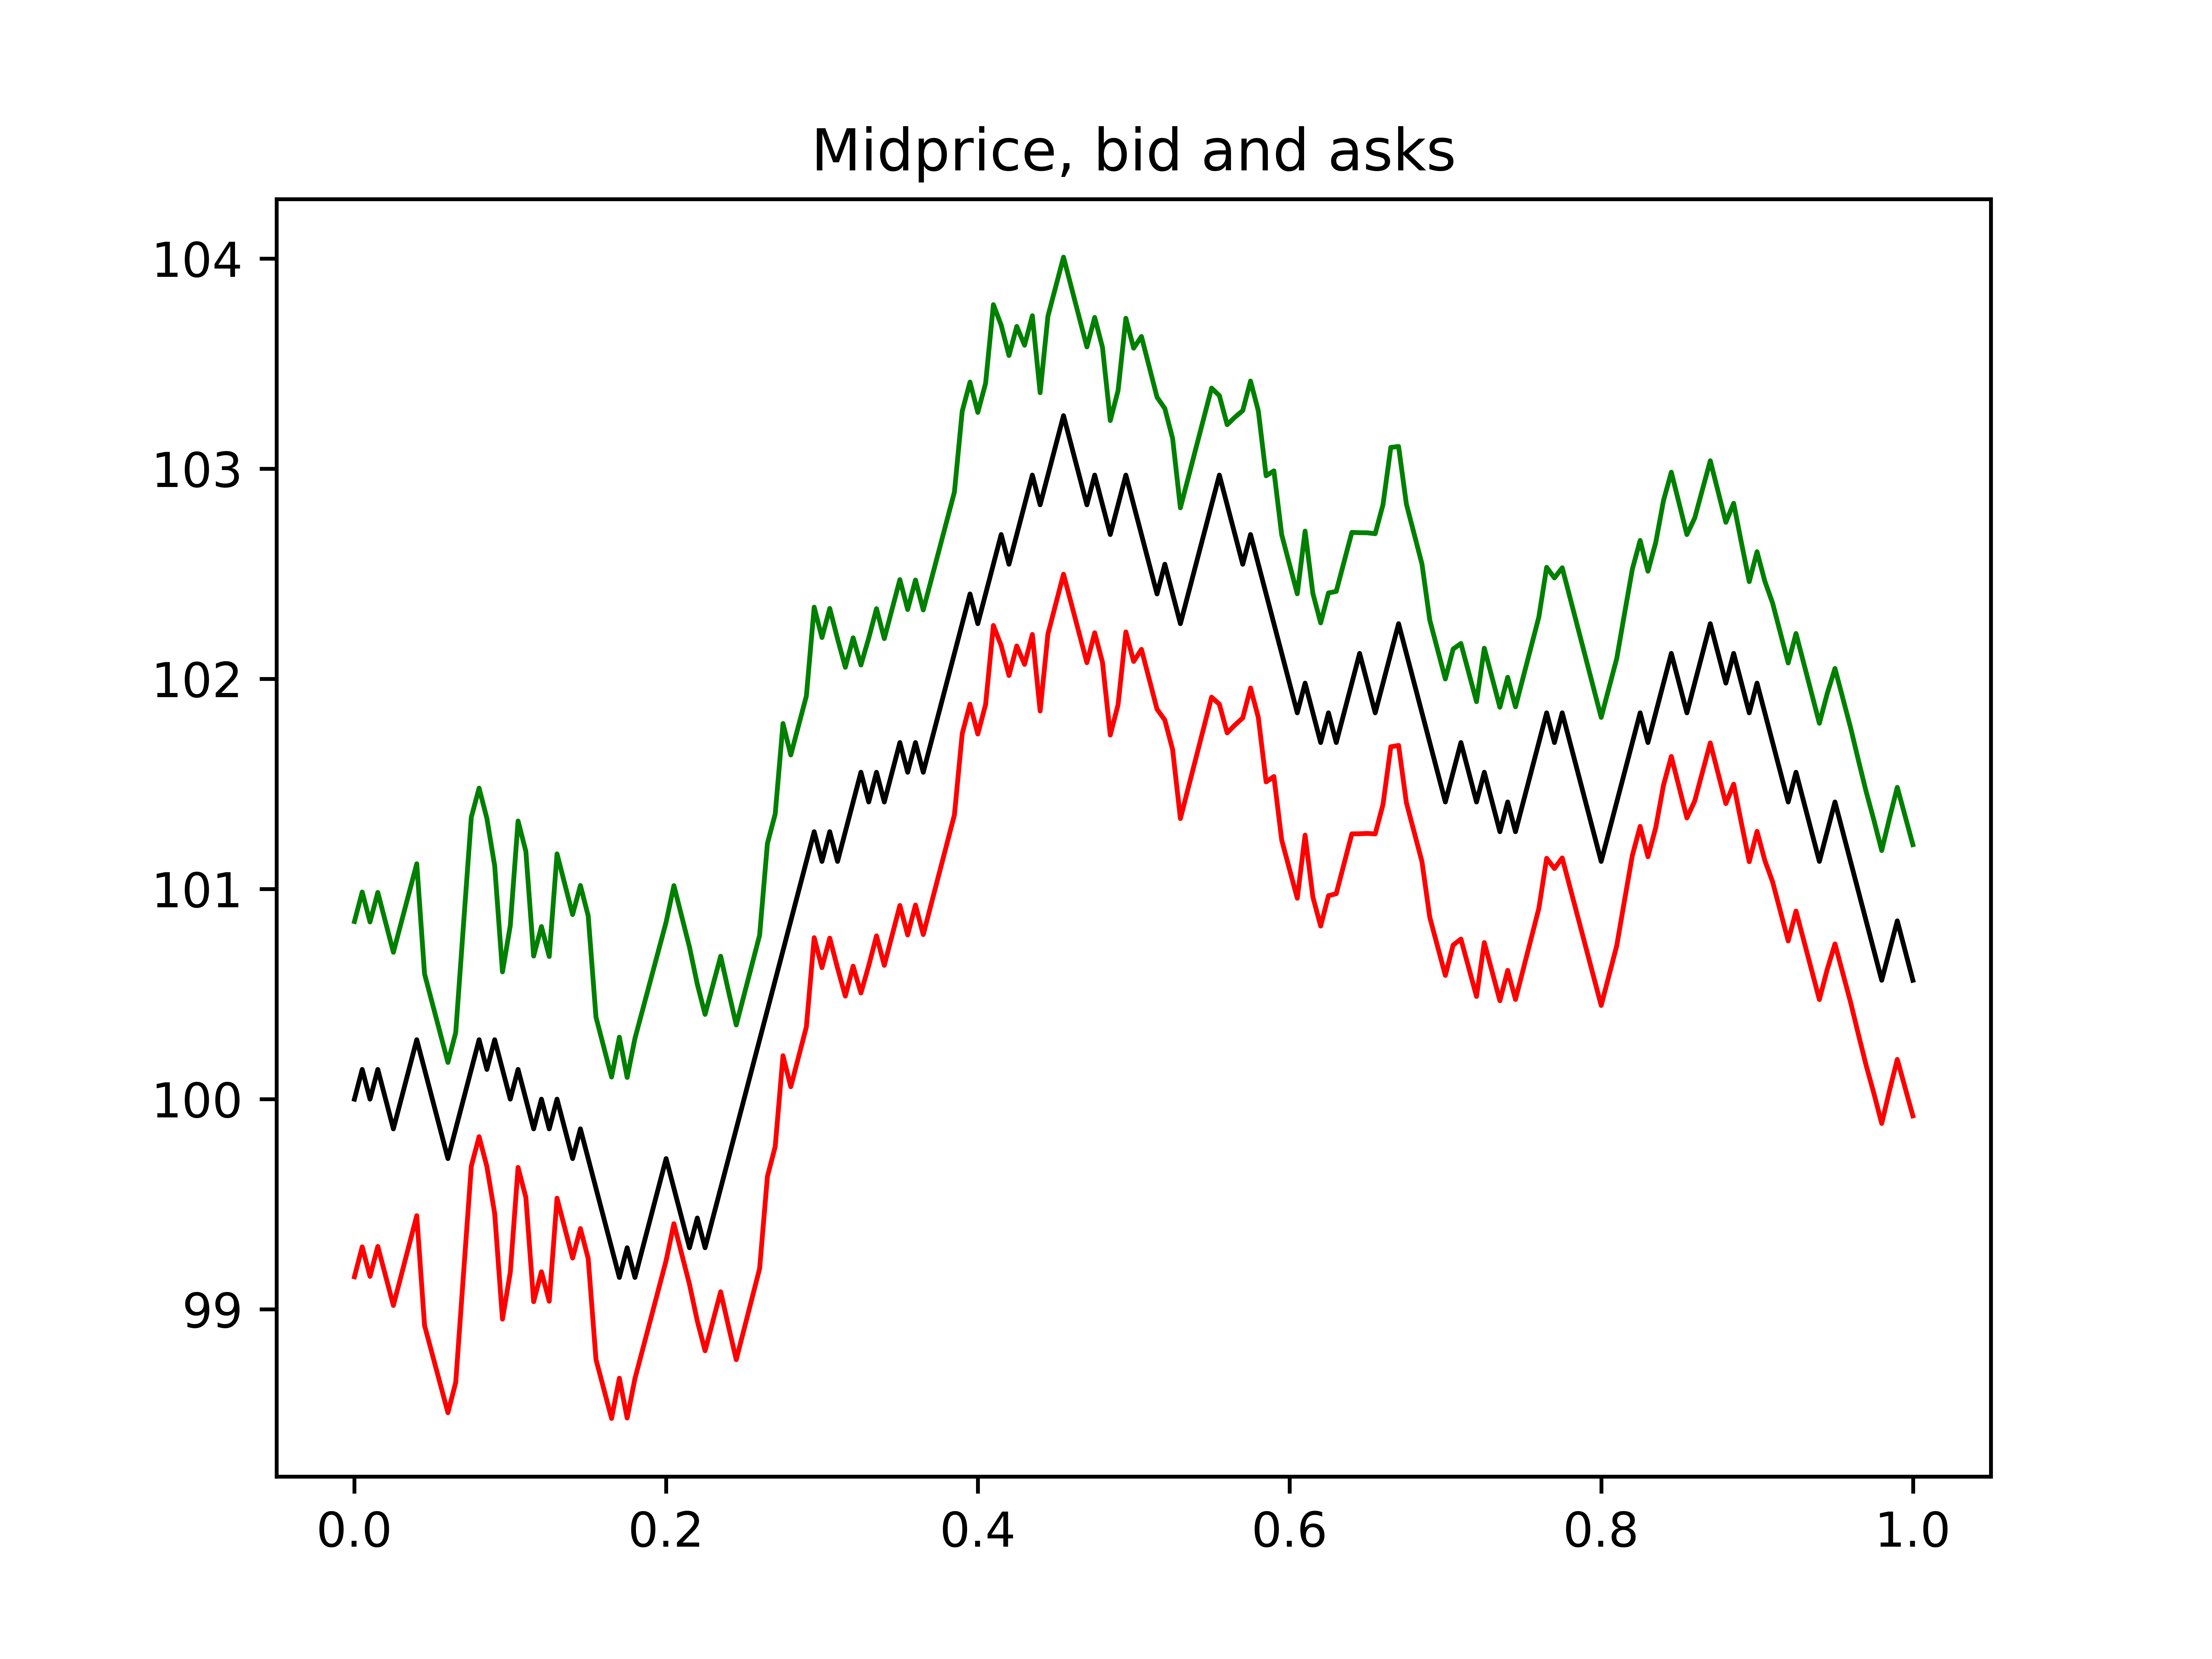
\includegraphics[height=5cm, width=7cm]{./plot.png}
    }
\end{frame}

% Conclusion
\begin{frame}{Conclusion}
    \begin{itemize}
        \item Stochastic control provides a useful framework through which to analyse the behaviour of market participants
        \item We can apply this framework to model the optimal behaviour of a dealer in financial markets
        \item This behaviour depends on the statistical properties of the particular market, which we can infer from market data
    \end{itemize}
\end{frame}

% Thank you & questions slide
\begin{frame}
    \frametitle{}
    \begin{center}
        \large{Thank you for your attention!}\\
        \vspace{1cm}
        Questions?
        \vspace{2cm}

        email: \texttt{josh.acton.2021@bristol.ac.uk}
    \end{center}
\end{frame}

\end{document}
